\section{Explain the difference between introspection and intercession. Which of these is mostly
supported by Java’s reflection API?}

\textbf{Reification } is the process of making a domain/language entity accessible to the program, so that it can be manipulated by computation.
The difference between \textbf{introspection} and \textbf{intercession} lies in the fact that \textbf{introspection} is the process of examining reified entitites (obtained by reification). It can be assimilated as an  "\textit{read only}" access. Whereas \textbf{intercession} is the process of manipulating reified entities. We intervene in the program execution. \\

Introspection is mostly supported by Java's reflection API as it contains a rich set of operations for it in contrast to intercession.

\section{Discuss (with a concrete example) how reflective programming could be used to make a
program more adaptable.}

The code below show an example on how reflective programming could be used to make a program more adaptable. The problem is that we have a bunch of classes representing visual components which do not share a common supertype or interface (the reasons may be that they come from different libraries). The only common base class is \textit{Object}. However, they all contains the same method \textbf{setColor(Color a Color)}  which we desire to call. \\

Reflective programming is an elegant and maintanable solution to that problem as the methode \textbf{setObjectColor} can be used on any components that contains the method  \textbf{setColor(Color a Color)}. There exists other solutions (using instanceOf and casting, adapter for each component, ...) but they all have as drawbacks that if we create another component class, the code must be changed to be able to call  \textbf{setColor(Color a Color)} on this new class.

\begin{lstlisting}[caption=reflective program]
public class Main {

    static Object[] components = new Object[10];
    static Color coler = new Color(0);
    
    public static void initializeComponents(){
      components[0] = new Component1();
      components[1] = new Component2();
      ...
    }
    
    public static void main(String[] args){
      initializeComponents();
      for(int i =0; i < args.length; i++){
        if(components[i] != null)
           setObjectColor(components[i], color);    //reflective method
      }
    }
    
    public static void setObjectColor(Object obj, Color color){
      Class cls = obj.getClass();
      try{
        Method method = cls.getMethod("setCOlor", new Class[]{Color.class});   // query the "setColor" method
        method.invoke(obj, new Object[]{color});   // invoke the method "setColor" with color as argument
      } catch(NoSuchMethodException ex){ 
        ..
      }catch(IllegalAccessException ex){
        ..
      }catch(InvocationTargetException ex){
        ..
      }
    }
}
\end{lstlisting}

\section{What are the possible problems of reflection with respect to maintainability?}

The possible problems of reflection with respect to maintainability are:
\begin{itemize}
\item You lose compile-time type safety which makes reflective program more error prone.This leads to having to handle all possible exceptions that may arise from it.
\item You may expose some internals by accessing private fields.
\item Reflective programming reduce the performance.
\end{itemize}


\section{In Java’s meta-object protocol, what does the class Object represent?
What happens when you ask Object for its class?
What Java instruction can you use to retrieve that class?}

In Java's meta-object protocol, the class \textit{Object} is the base class. It means that all other classes are subclass of \textit{Object}. \\

When asking for the class of the class Object, it returns the meta class \textit{Class}.  The Java instructions use to retrieve that class is :  \textbf{getClass}.

\begin{figure}[!ht]
	\centering
	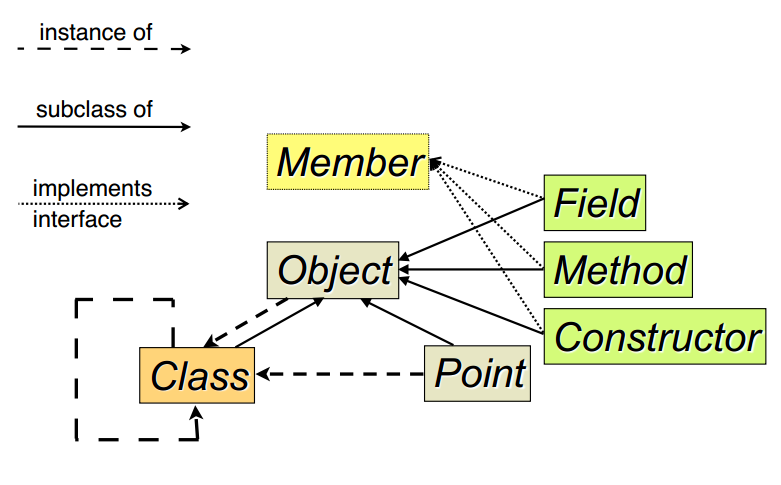
\includegraphics[scale=0.5]{meta.PNG}
\end{figure}
\FloatBarrier{}

\section{In Java’s meta-object protocol, what does the class Class represent?
What happens when you ask this class for its class?
What Java instruction can you use to do that?}

In Java's meta-object protocol, the meta class \textbf{Class} is the class of all classes. It means that all classes are instances of it. \\
If you ask the class \textbf{Class} for it's class, it will return itself. The Java instruction that you can use if the following one :  \textbf{getClass}.

\begin{figure}[!ht]
	\centering
	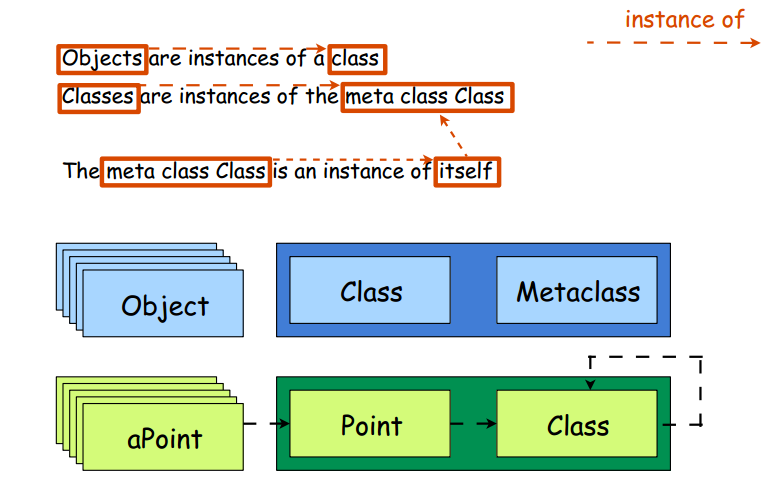
\includegraphics[scale=0.5]{instance.PNG}
\end{figure}
\FloatBarrier{}

\section{How is the call stack reified in the Java reflection API?
What kind of reflection (intercession or introspection) can be used to manipulate this call
stack? Explain.}

In Java reflection API, the call stack is reified by accessing an array of \textbf{StackTraceElement}, which is created when an instance of \textbf{Throwable} is created. There is no accessible CallStack meta-object. This call stack can only be manipulated by \textbf{introspection}. We can only examine it. We cannot modify the call stack via the Java reflection API.
